\addcontentsline{toc}{section}{APÊNDICES}
\begin{center}
\section*{APÊNDICES}
\end{center}

Os apêndices a seguir apresentam informações complementares ao desenvolvimento e validação do sistema proposto. Os Apêndices A a F contêm os principais excertos do código-fonte desenvolvidos para a camada de serviços da aplicação, incluindo os algoritmos de dimensionamento e a suíte de testes unitários. Por sua vez, os Apêndices G a K reúnem as interfaces do sistema e os relatórios de cálculo estrutural gerados de forma automática pela aplicação.

% =========================================================
% APÊNDICE A
% =========================================================
\newpage
\addcontentsline{toc}{section}{APÊNDICE A - Serviço de Dimensionamento de Vigas (viga\_service.py)}
\begin{center}
\section*{APÊNDICE A}
Serviço de Dimensionamento de Vigas (viga\_service.py)
\end{center}

O excerto seguinte apresenta a função principal de dimensionamento de vigas à flexão simples. Destacam-se o cálculo iterativo da altura útil, a verificação do momento reduzido, a determinação da armadura necessária e a chamada ao serviço de otimização.

\newpage
\begin{lstlisting}[style=PythonStyle, basicstyle=\ttfamily\normalsize, caption={Excerto de viga\_service.py (Dimensionamento principal)}, label={lst:viga_service}]
# calculos/services/viga_service.py
import math
from . import armadura_service

def dimensionar_viga(b, h, f_ck, f_yk, M_Ed_kNm, c_nom):
    passos = []

    gamma_c, gamma_s, alpha_cc, lambda_val = 1.5, 1.15, 1.0, 0.8
    f_cd_mpa = alpha_cc * f_ck / gamma_c
    f_yd_mpa = f_yk / gamma_s
    M_Ed_Nm = M_Ed_kNm * 1000
    b_m = b / 1000
    phi_estribo = 8.0

    phi_long_assumido = 16.0
    d = h - c_nom - phi_estribo - (phi_long_assumido / 2)
    d_m = d / 1000

    mu = M_Ed_Nm / (b_m * d_m**2 * (f_cd_mpa * 10**6)) if (b_m * d_m**2 * f_cd_mpa) > 0 else 0

    mu_lim = lambda_val * 0.45 * (1 - 0.5 * lambda_val * 0.45)
    if mu > mu_lim:
        raise ValueError("A secção necessita de ser redimensionada.")

    xi_temp = (1 - math.sqrt(1 - 2 * mu)) / lambda_val if mu < 0.5 else 1.25
    z_temp = d_m * (1 - 0.5 * lambda_val * xi_temp)
    As_req_cm2_temp = (M_Ed_Nm / (z_temp * (f_yd_mpa * 10**6))) * 10000 if z_temp > 0 else 0

    largura_disponivel = b - 2 * c_nom - 2 * phi_estribo
    solucoes_temp = armadura_service.encontrar_combinacoes_otimas(
        As_req_cm2_temp, largura_disponivel
    )

    solucao_unica_temp = solucoes_temp.get('unica')
    phi_long_final = 0
    if solucao_unica_temp:
        phi_long_final = int(solucao_unica_temp['combinacao_str'].split('Ø')[1])

    if phi_long_final and phi_long_final != phi_long_assumido:
        d = h - c_nom - phi_estribo - (phi_long_final / 2)
        d_m = d / 1000
        mu = M_Ed_Nm / (b_m * d_m**2 * (f_cd_mpa * 10**6)) if (b_m * d_m**2 * f_cd_mpa) > 0 else 0

    xi = (1 - math.sqrt(1 - 2 * mu)) / lambda_val if mu < 0.5 else 1.25
    z = d_m * (1 - 0.5 * lambda_val * xi)
    As_req_cm2 = (M_Ed_Nm / (z * (f_yd_mpa * 10**6))) * 10000 if z > 0 else 0

    solucoes = armadura_service.encontrar_combinacoes_otimas(
        As_req_cm2, largura_disponivel
    )

    solucao_unica = solucoes.get('unica')
    solucao_mista = solucoes.get('mista')

    if solucao_unica and solucao_mista:
        solucao_principal = min(
            [solucao_unica, solucao_mista],
            key=lambda x: x['area_total_cm2']
        )
    else:
        solucao_principal = solucao_unica or solucao_mista

    combinacao_final_str = solucao_principal['combinacao_str']
    As_prov_cm2 = solucao_principal['As_final_cm2']

    return {
        'status': 'Sucesso',
        'combinacao_final': combinacao_final_str,
        'As_final_cm2': f"{As_prov_cm2:.2f}"
    }
\end{lstlisting}

% =========================================================
% APÊNDICE B
% =========================================================
\newpage
\addcontentsline{toc}{section}{APÊNDICE B - Serviço de Dimensionamento de Pilares (pilar\_service.py)}
\begin{center}
\section*{APÊNDICE B}
Serviço de Dimensionamento de Pilares (pilar\_service.py)
\end{center}

O excerto abaixo mostra a lógica principal do \texttt{pilar\_service.py}, incluindo a verificação de esbelteza, a consideração dos efeitos de segunda ordem e a chamada ao método iterativo rigoroso de dimensionamento.

\newpage
\begin{lstlisting}[style=PythonStyle, basicstyle=\ttfamily\normalsize, caption={Excerto de pilar\_service.py (Dimensionamento principal)}, label={lst:pilar_service}]
# calculos/services/pilar_service.py
import math
from . import armadura_service

def dimensionar_pilar(b_mm, h_mm, l_m, lig_topo, lig_base,
                      f_ck, f_yk, N_Ed_kN, M0_Ed_kNm,
                      c_nom_mm, phi_ef):

    passos = []
    phi_estribo = 8.0

    gamma_c, gamma_s, alpha_cc = 1.5, 1.15, 1.0
    f_cd_mpa = alpha_cc * f_ck / gamma_c
    f_yd_mpa = f_yk / gamma_s

    N_Ed_N = N_Ed_kN * 1000
    M0_Ed_Nm = M0_Ed_kNm * 1000
    Ac_mm2 = b_mm * h_mm

    beta = 1.0
    l0_m = beta * l_m
    i_mm = h_mm / math.sqrt(12)
    esbelteza = (l0_m * 1000) / i_mm if i_mm > 0 else 0

    n = N_Ed_N / (Ac_mm2 * f_cd_mpa) if (Ac_mm2 * f_cd_mpa) > 0 else 0
    A = 1 / (1 + 0.2 * phi_ef)
    B, C = 1.1, 0.7
    lambda_lim = 20 * A * B * C / math.sqrt(n) if n > 0 else float('inf')

    M_Ed_total_Nm = M0_Ed_Nm

    if esbelteza > lambda_lim:
        As_est_mm2 = max(0.10 * N_Ed_N / f_yd_mpa, 0.002 * Ac_mm2)
        Es_mpa = 200000
        M2_Ed_Nm, e2_mm, inv_r, omega, K_r, beta_creep, K_phi, inv_r0, d_estimado_mm = \
            calcular_momento_segunda_ordem(
                esbelteza, f_ck, f_yd_mpa, f_cd_mpa, Es_mpa,
                N_Ed_N, Ac_mm2, As_est_mm2, l0_m, h_mm,
                c_nom_mm, phi_estribo, phi_ef, n
            )
        M_Ed_total_Nm = M0_Ed_Nm + M2_Ed_Nm

    As_req_mm2_final, MRd_kNm, x_final = _dimensionar_pilar_rigoroso(
        b_mm, h_mm, f_ck, f_cd_mpa, f_yd_mpa,
        N_Ed_N, M_Ed_total_Nm, c_nom_mm, passos
    )

    As_min_cm2_1 = 0.10 * N_Ed_N / f_yd_mpa / 100
    As_min_cm2_2 = 0.002 * Ac_mm2 / 100
    As_min_cm2 = max(As_min_cm2_1, As_min_cm2_2)
    As_final_req_cm2 = max(As_req_mm2_final / 100, As_min_cm2)

    largura_disponivel = h_mm - 2 * c_nom_mm - 2 * phi_estribo
    solucoes = armadura_service.encontrar_combinacoes_otimas_pilar(
        As_final_req_cm2, largura_disponivel, b_mm, h_mm
    )

    solucao_unica = solucoes.get('unica')
    solucao_mista = solucoes.get('mista')
    solucao_principal = solucao_unica or solucao_mista

    return {
        'status': 'Sucesso',
        'combinacao_final': solucao_principal['combinacao_str'],
        'As_final_cm2': f"{solucao_principal['As_final_cm2']:.2f}"
    }
\end{lstlisting}

% =========================================================
% APÊNDICE C
% =========================================================
\newpage
\addcontentsline{toc}{section}{APÊNDICE C - Serviço de Dimensionamento de Sapatas (sapata\_service.py)}
\begin{center}
\section*{APÊNDICE C}
Serviço de Dimensionamento de Sapatas (sapata\_service.py)
\end{center}

O excerto seguinte demonstra a dupla iteração implementada no \texttt{sapata\_service.py}: numa primeira fase são definidas as dimensões em planta por verificação geotécnica em ELS e, numa segunda fase, é determinada a altura resistente por verificação estrutural ao punçoamento em ELU.

\newpage
\begin{lstlisting}[style=PythonStyle, basicstyle=\ttfamily\normalsize, caption={Excerto de sapata\_service.py (Dupla iteração)}, label={lst:sapata_service}]
# calculos/services/sapata_service.py
import math

def dimensionar_sapata(sigma_adm_kpa, f_ck, f_yk, c_nom_mm,
                       bp_mm, hp_mm, N_Ed_kN, M_Edy_kNm):
    passos = []
    gamma_g_avg = 1.4

    N_k_kN = N_Ed_kN / gamma_g_avg
    M_ky_kNm = M_Edy_kNm / gamma_g_avg

    A_req_preliminar = N_k_kN / sigma_adm_kpa if sigma_adm_kpa > 0 else 1.0
    A_majorada = A_req_preliminar * 1.2

    if bp_mm == hp_mm:
        A_m = math.sqrt(A_majorada)
        B_m = A_m
    else:
        proporcao = hp_mm / bp_mm if bp_mm > 0 else 1
        A_m = math.sqrt(A_majorada / proporcao)
        B_m = A_m * proporcao
    for i in range(50):
        H_estimado_m = max(A_m, B_m) / 8 if max(A_m, B_m) / 8 > 0.4 else 0.4
        W_k_kN = A_m * B_m * H_estimado_m * 25
        N_total_k_kN = N_k_kN + W_k_kN
        e_y_m = M_ky_kNm / N_total_k_kN if N_total_k_kN > 0 else 0

        sigma_max_kpa_real = (N_total_k_kN / (A_m * B_m)) * (1 + 6 * e_y_m / B_m)
        sigma_min_kpa_real = (N_total_k_kN / (A_m * B_m)) * (1 - 6 * e_y_m / B_m)

        if e_y_m > B_m / 6:
            B_m += 0.05
            A_m = B_m * (bp_mm / hp_mm) if hp_mm > 0 else B_m
            continue

        if sigma_max_kpa_real <= sigma_adm_kpa and sigma_min_kpa_real >= 0:
            break

        B_m += 0.05
        A_m = B_m * (bp_mm / hp_mm) if hp_mm > 0 else B_m
    A_final_m = math.ceil(A_m * 20) / 20
    B_final_m = math.ceil(B_m * 20) / 20
    d_m = 0.15
    for i in range(50):
        # calculo de puncoamento
        if VRd_c_pun_kN > V_Ed_pun_kN:
            H_final_mm = math.ceil((d_m + ... ) * 1000 / 50) * 50
            break
        d_m += 0.01
    # escolha de armaduras nas direcoes X e Y
    return resultado
\end{lstlisting}

% =========================================================
% APÊNDICE D
% =========================================================
\newpage
\addcontentsline{toc}{section}{APÊNDICE D - Serviço de Otimização de Armaduras (armadura\_service.py)}
\begin{center}
\section*{APÊNDICE D}
Serviço de Otimização de Armaduras (armadura\_service.py)
\end{center}

O serviço \texttt{armadura\_service.py} centraliza a lógica de seleção de combinações de varões para vigas e pilares. O algoritmo gera combinações válidas, verifica o espaçamento mínimo e seleciona a solução de menor área que satisfaça a área requerida.

\newpage
\begin{lstlisting}[style=PythonStyle, basicstyle=\ttfamily\normalsize, caption={Excerto de armadura\_service.py (Otimização de armaduras)}, label={lst:armadura_service}]
# calculos/services/armadura_service.py
import math
from itertools import combinations_with_replacement

VERGALHOES_PADRAO = {
    10: 0.785,
    12: 1.131,
    16: 2.011,
    20: 3.142,
    25: 4.909,
    32: 8.042,
    40: 12.566,
    50: 19.635,
    55: 23.758,
    60: 28.274,
}

def _verificar_espacamento(combinacao, largura_disponivel):
    num_barras = len(combinacao)
    if num_barras <= 1:
        return True
    espacamento_minimo_horizontal = max(max(combinacao), 20)
    largura_necessaria = sum(combinacao) + (num_barras - 1) * espacamento_minimo_horizontal
    return largura_necessaria <= largura_disponivel

def encontrar_combinacoes_otimas(As_req_cm2, largura_disponivel_mm, tipo_elemento="viga"):
    solucoes_unicas = []
    solucoes_mistas = []
    diametros = sorted(list(VERGALHOES_PADRAO.keys()))
    max_barras = 8
    todas_as_combinacoes = []

    for num_barras in range(2, max_barras + 1):
        for diametro in diametros:
            todas_as_combinacoes.append(tuple([diametro] * num_barras))

        if num_barras >= 4 and num_barras % 2 == 0:
            pares_de_diametros = list(combinations_with_replacement(diametros, 2))
            for d1, d2 in pares_de_diametros:
                if d1 == d2:
                    continue
                for i in range(1, num_barras // 2):
                    if (num_barras - 2 * i) == i * 2:
                        break
                    comb = tuple(sorted([d1] * (i * 2) + [d2] * (num_barras - i * 2)))
                    todas_as_combinacoes.append(comb)

    todas_as_combinacoes = sorted(list(set(todas_as_combinacoes)), key=lambda x: (len(x), sum(x)))

    for comb in todas_as_combinacoes:
        if _verificar_espacamento(comb, largura_disponivel_mm):
            area_total_cm2 = sum(VERGALHOES_PADRAO[d] for d in comb)
            if area_total_cm2 >= As_req_cm2:
                counts = {d: comb.count(d) for d in set(comb)}
                combinacao_str = " + ".join([f"{count} Ø {diam}" for diam, count in sorted(counts.items())])

                if len(counts) > 1:
                    solucoes_mistas.append({"combinacao_str": combinacao_str, "area_total_cm2": area_total_cm2})
                else:
                    solucoes_unicas.append({"combinacao_str": combinacao_str, "area_total_cm2": area_total_cm2})

    melhor_unica = min(solucoes_unicas, key=lambda x: x["area_total_cm2"]) if solucoes_unicas else None
    melhor_mista = min(solucoes_mistas, key=lambda x: x["area_total_cm2"]) if solucoes_mistas else None

    return {
        "unica": melhor_unica,
        "mista": melhor_mista
    }

def encontrar_combinacoes_otimas_pilar(As_req_cm2, largura_disponivel_mm, b_mm=None, h_mm=None):
    # logica especifica para pilares: numero par de varoes e simetria
    pass
\end{lstlisting}

% =========================================================
% APÊNDICE E
% =========================================================
\newpage
\addcontentsline{toc}{section}{APÊNDICE E - Funções de Geração SVG}
\begin{center}
\section*{APÊNDICE E}
Funções de Geração SVG
\end{center}

Para além dos cálculos numéricos, a aplicação gera automaticamente representações gráficas em SVG das secções dimensionadas. Seguem-se excertos resumidos das funções responsáveis pela geração das vistas de viga, pilar e sapata.

\newpage
\begin{lstlisting}[style=PythonStyle, basicstyle=\ttfamily\normalsize, caption={Funções de desenho SVG dos elementos estruturais}, label={lst:svg_services}]
# viga_service.py
def desenhar_viga_svg(dados_desenho):
    b = dados_desenho.get('b', 300) ; h = dados_desenho.get('h', 500)
    c_nom = dados_desenho.get('c_nom', 30)
    phi_estribo = dados_desenho.get('phi_estribo', 8)
    n_barras = dados_desenho.get('n_barras', 0)
    phi_long = dados_desenho.get('phi_long', 0)
    PADDING = 60
    estribo_x = PADDING + c_nom
    estribo_y = PADDING + c_nom
    estribo_w = b - 2 * c_nom
    estribo_h = h - 2 * c_nom
    if n_barras > 0 and phi_long > 0:
        y_pos_inf = PADDING + h - c_nom - phi_estribo - (phi_long / 2)
        start_x_inf = estribo_x + (phi_estribo / 2) + (phi_long / 2)
        available_width = estribo_w - phi_estribo - phi_long
        for i in range(n_barras):
            x_pos = start_x_inf
            if n_barras > 1:
                x_pos += i * (available_width / (n_barras - 1))
    return svg
# pilar_service.py
def desenhar_pilar_svg(dados_desenho):
    b = dados_desenho.get('b', 300) ; h = dados_desenho.get('h', 400)
    c_nom = dados_desenho.get('c_nom', 35)
    phi_estribo = dados_desenho.get('phi_estribo', 8)
    n_barras = dados_desenho.get('n_barras', 4)
    phi_long = dados_desenho.get('phi_long', 16)
    if n_barras > 0 and phi_long > 0:
        canto_sup_esq = (estribo_x + phi_long/2, estribo_y + phi_long/2)
        canto_sup_dir = (estribo_x + estribo_w - phi_long/2, estribo_y + phi_long/2)
        canto_inf_esq = (estribo_x + phi_long/2, estribo_y + estribo_h - phi_long/2)
        canto_inf_dir = (estribo_x + estribo_w - phi_long/2, estribo_y + estribo_h - phi_long/2)
        posicoes = [canto_sup_esq, canto_sup_dir, canto_inf_esq, canto_inf_dir]
    return svg
# sapata_service.py
def desenhar_sapata_planta_svg(dados_desenho):
    A = dados_desenho['A_m'] ; B = dados_desenho['B_m']
    bp = dados_desenho['bp_mm'] / 1000
    hp = dados_desenho['hp_mm'] / 1000
    phi_x = dados_desenho['phi_x']
    phi_y = dados_desenho['phi_y']
    return svg
def desenhar_sapata_corte_svg(dados_desenho):
    A = dados_desenho['A_m']
    H = dados_desenho['H_mm'] / 1000
    bp = dados_desenho['bp_mm'] / 1000
    return svg
\end{lstlisting}

% =========================================================
% APÊNDICE F
% =========================================================
\newpage
\addcontentsline{toc}{section}{APÊNDICE F - Testes Unitários (calculos/tests.py)}
\begin{center}
\section*{APÊNDICE F}
Testes Unitários (calculos/tests.py)
\end{center}

Este excerto apresenta os testes unitários automatizados usados para validar os serviços de vigas, pilares e sapatas. Cada teste define um conjunto conhecido de entradas e compara os resultados obtidos com valores esperados.

\newpage
\begin{lstlisting}[style=PythonStyle, basicstyle=\ttfamily\normalsize, caption={Testes Unitários Automatizados (calculos/tests.py)}, label={lst:tests_py}]
# calculos/tests.py
from django.test import TestCase
from .services import viga_service, pilar_service, sapata_service

# TESTES PARA O SERVIÇO DE VIGAS
class VigaServiceTests(TestCase):
    
    def test_dimensionamento_viga_cenario_tipico(self):
        "Testa o dimensionamento de viga com um resultado de di^ametro único."
        print("\n=> Executando teste para o dimensionamento de viga (cenário típico)...")
        dados_viga = {
            "b": 300, "h": 500, "f_ck": 25, "f_yk": 500,
            "M_Ed_kNm": 150, "c_nom": 35
        }
        resultado = viga_service.dimensionar_viga(**dados_viga)
        self.assertEqual(resultado['status'], 'Sucesso')
        # CORREÇÃO FINAL: Atualizado para o resultado verdadeiramente ótimo encontrado pelo algoritmo
        self.assertEqual(resultado['combinacao_final'], '4 Ø 12 + 2 Ø 16')
        self.assertAlmostEqual(float(resultado['As_final_cm2']), 8.55, places=2)
        print("   Teste da viga (cenário típico) concluído com sucesso!")

    def test_dimensionamento_viga_combinacao_mista(self):
        """Testa o dimensionamento de viga onde a solução ótima é uma combinação mista."""
        print("\n=> Executando teste para o dimensionamento de viga (combinação mista)...")
        dados_viga = {
            "b": 350, "h": 600, "f_ck": 30, "f_yk": 500,
            "M_Ed_kNm": 350, "c_nom": 35
        }
        resultado = viga_service.dimensionar_viga(**dados_viga)
        self.assertEqual(resultado['status'], 'Sucesso')
        # Este resultado já estava correto na execução anterior
        self.assertEqual(resultado['combinacao_final'], '2 Ø 16 + 4 Ø 20')
        self.assertAlmostEqual(float(resultado['As_final_cm2']), 16.59, places=2)
        print("   Teste da viga (combinação mista) concluído com sucesso!")

# TESTES PARA O SERVIÇO DE PILARES
class PilarServiceTests(TestCase):

    def test_dimensionamento_pilar_cenario_tipico(self):
        print("\n=> Executando teste para o dimensionamento de pilar...")
        dados_pilar = {
            "b_mm": 300, "h_mm": 400, "l_m": 3.5,
            "lig_topo": "artic", "lig_base": "artic",
            "f_ck": 25, "f_yk": 500,
            "N_Ed_kN": 800, "M0_Ed_kNm": 60,
            "c_nom_mm": 35, "phi_ef": 2.0
        }
        resultado = pilar_service.dimensionar_pilar(**dados_pilar)
        self.assertEqual(resultado['status'], 'Sucesso')
        # CORREÇ~{A}O FINAL: Adicionado o espaço para corresponder a nova formata\\c{c}~{a}o
        self.assertEqual(resultado['combinacao_final'], '4 Ø 10')
        self.assertAlmostEqual(float(resultado['As_final_cm2']), 3.14, places=2)
        print("   Teste do pilar concluído com sucesso!")

# TESTES PARA O SERVIÇO DE SAPATAS
class SapataServiceTests(TestCase):

    def test_dimensionamento_sapata_cenario_tipico(self):
        """
        Testa o cálculo de uma sapata com valores conhecidos.
        """
        print("\n=> Executando teste para o dimensionamento de sapata...")

        dados_sapata = {
            "sigma_adm_kpa": 200, "f_ck": 25, "f_yk": 500,
            "c_nom_mm": 50, "bp_mm": 400, "hp_mm": 400,
            "N_Ed_kN": 1200, "M_Edy_kNm": 60
        }
        resultado = sapata_service.dimensionar_sapata(**dados_sapata)
        self.assertEqual(resultado['status'], 'Sucesso')
        self.assertEqual(resultado['dimensoes'], '2.30m x 2.30m x 0.45m')
        self.assertEqual(resultado['armadura_x'], '14"\\diameter"12 (s \approx 168 mm)')
        self.assertEqual(resultado['armadura_y'], '14"\\diameter"12 (s \approx 168 mm)')
        print("   Teste da sapata concluído com sucesso!")
\end{lstlisting}

% =========================================================
% APÊNDICE G
% =========================================================
\newpage
\addcontentsline{toc}{section}{APÊNDICE G - Interface do Histórico de Cálculos}
\begin{center}
\section*{APÊNDICE G}
Interface do Histórico de Cálculos
\end{center}

O documento seguinte apresenta a interface do histórico de cálculos.

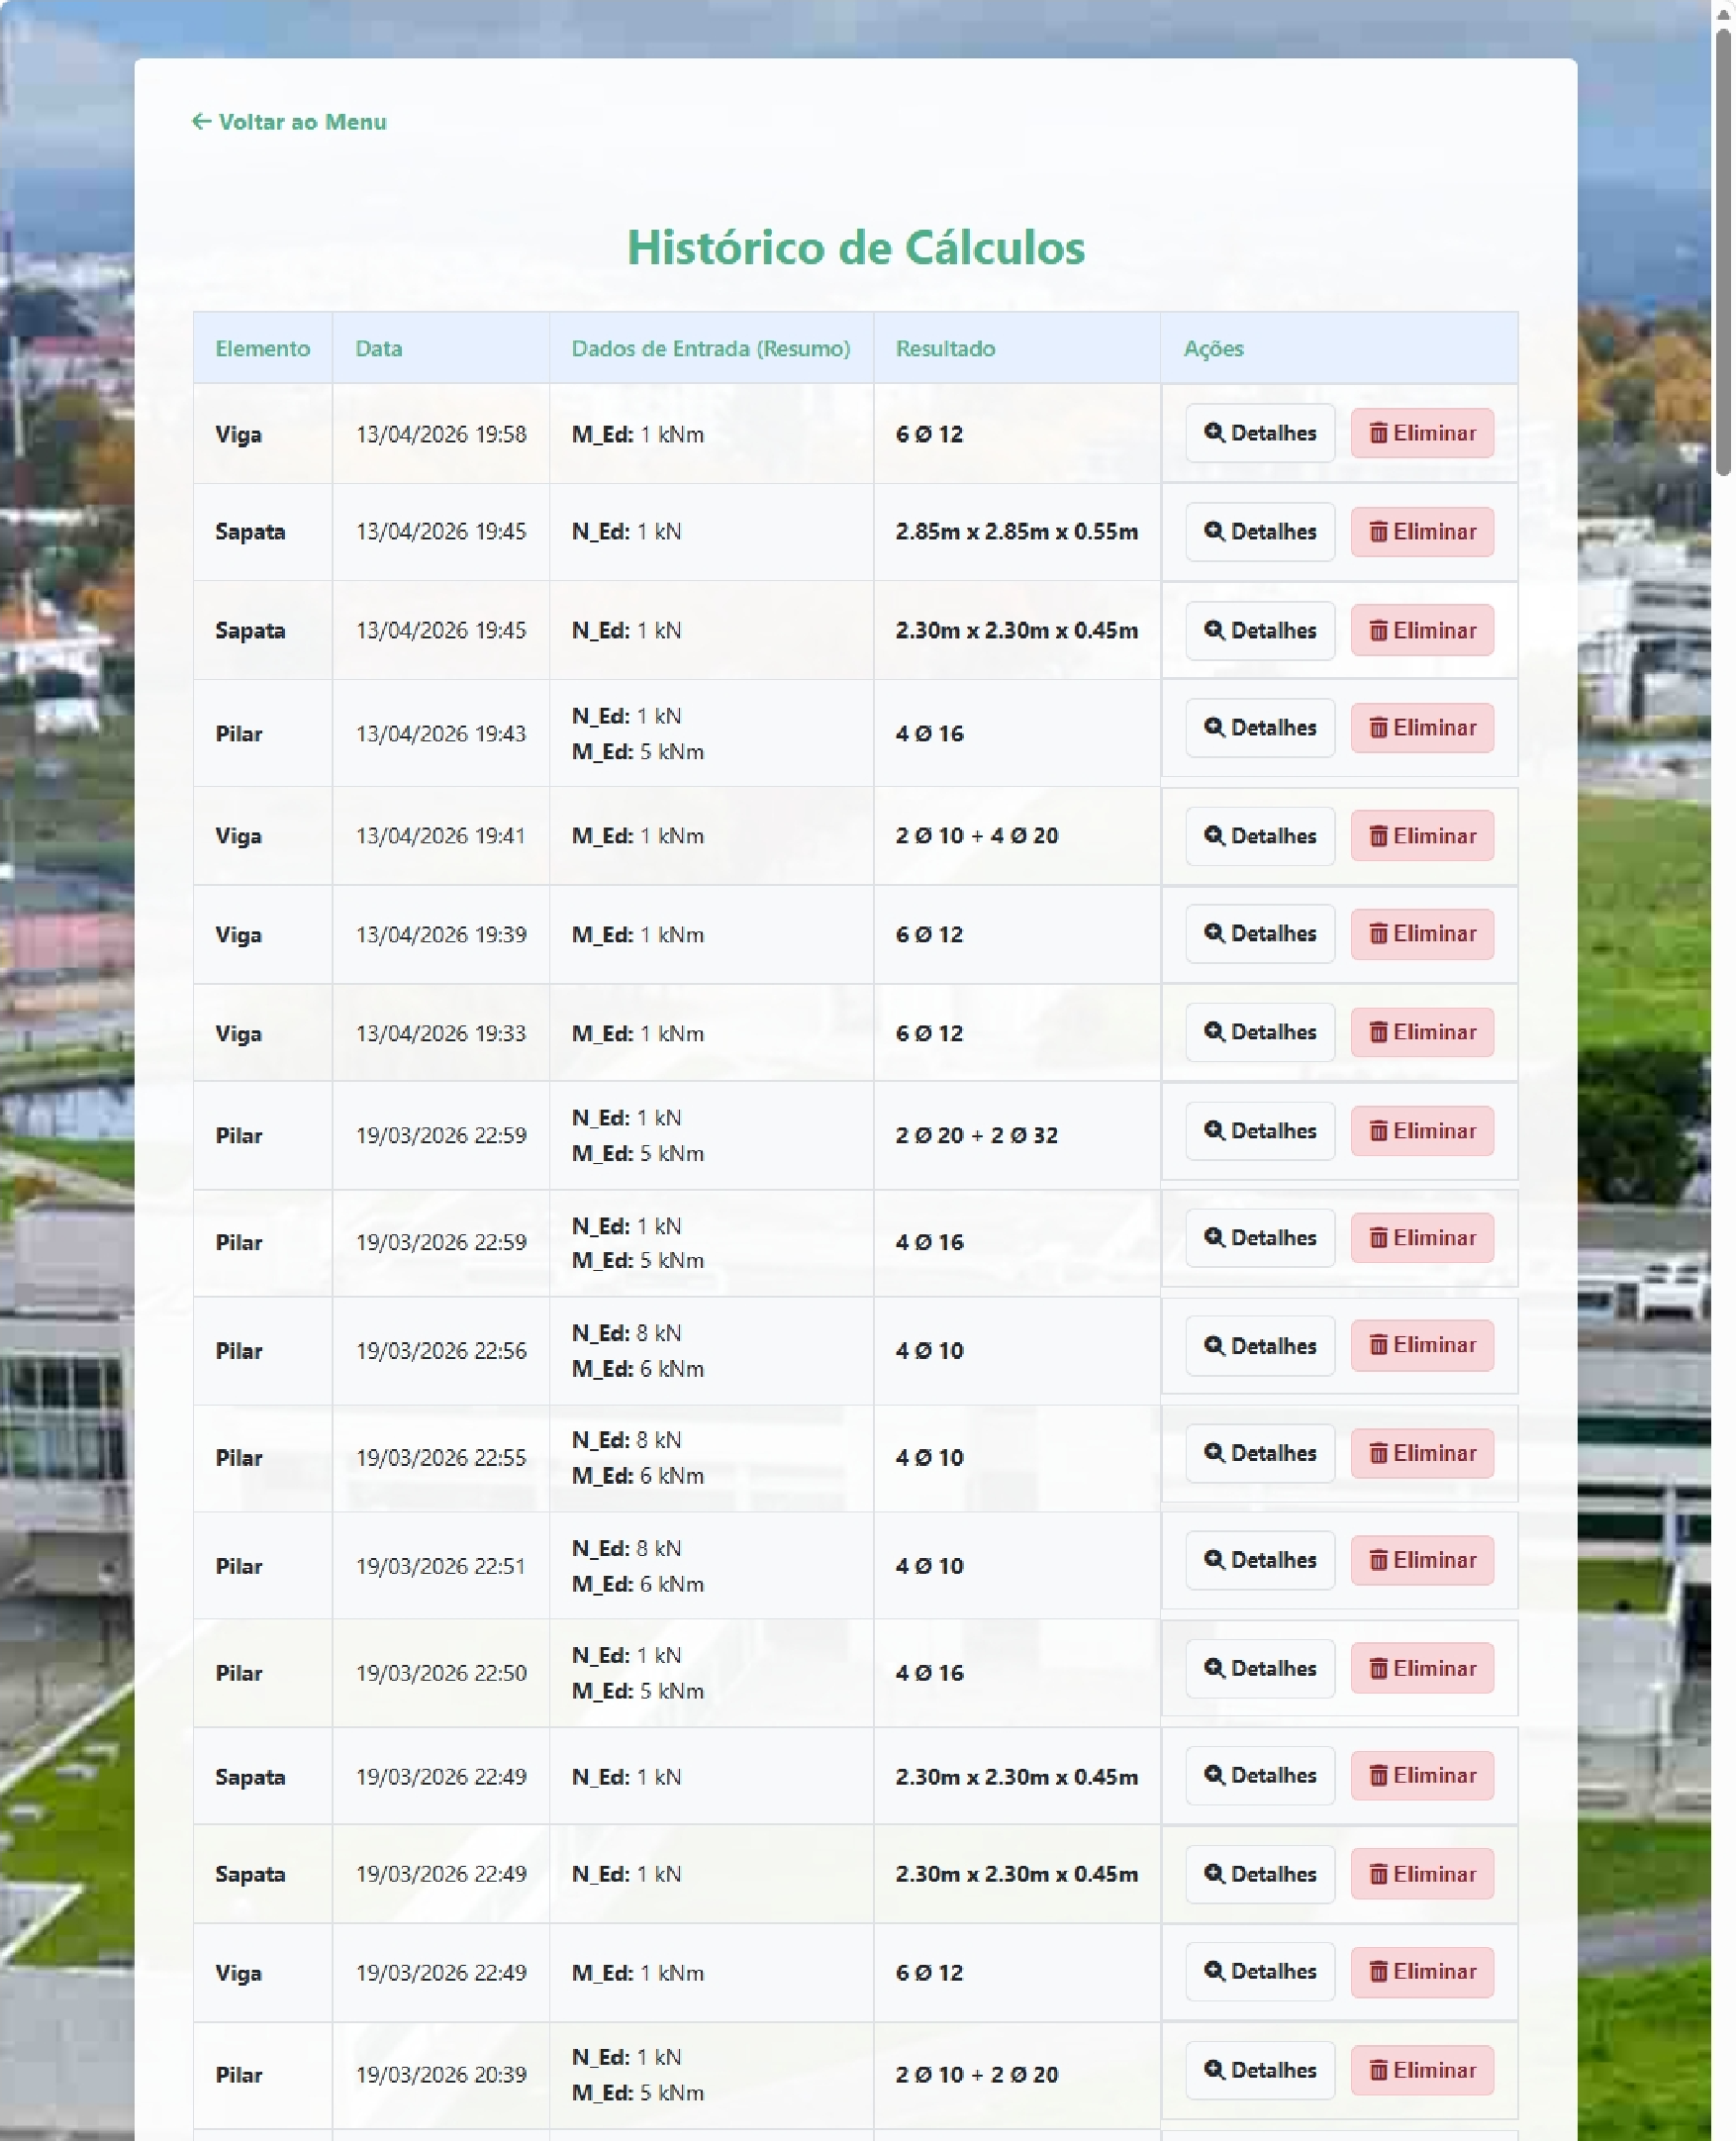
\includepdf[pages=-, pagecommand={}]{Anexos/Interface do histórico de cálculos.pdf}

% =========================================================
% APÊNDICE H
% =========================================================
\newpage
\addcontentsline{toc}{section}{APÊNDICE H - Interface de Configuração do Sistema}
\begin{center}
\section*{APÊNDICE H}
Interface de Configuração do Sistema
\end{center}

O documento seguinte apresenta a interface de configuração do sistema.

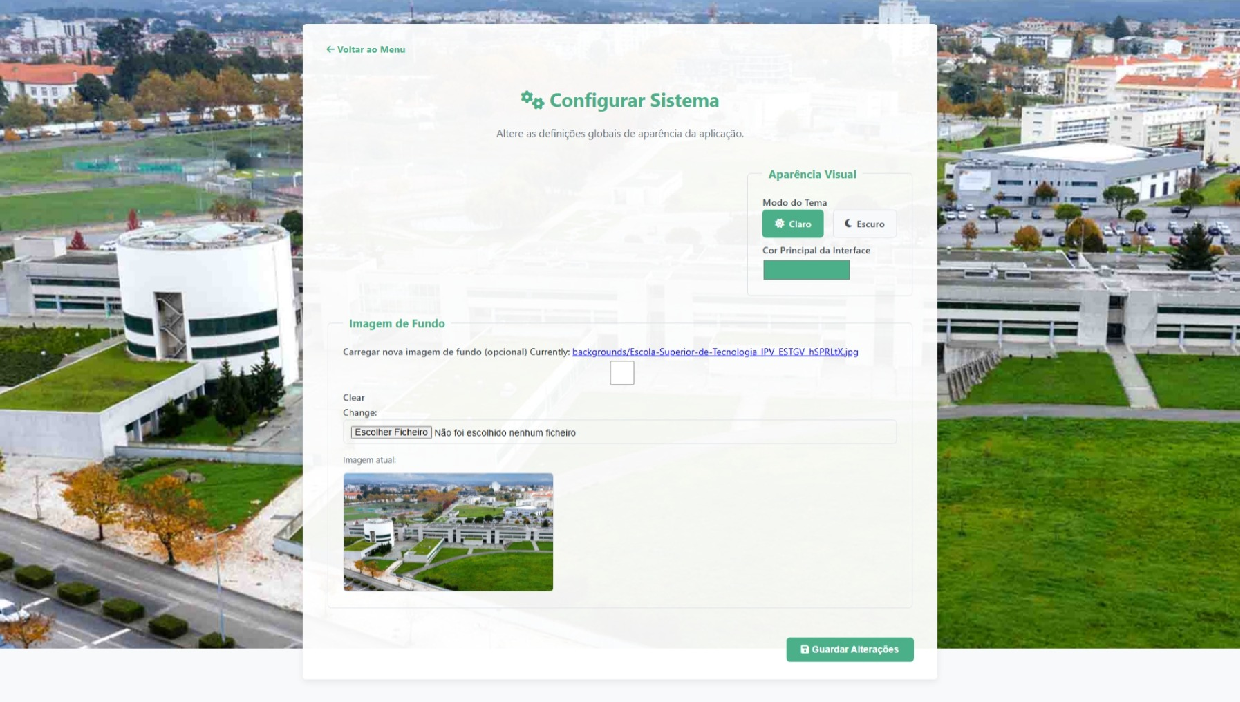
\includepdf[pages=-, pagecommand={}, angle=90]{Anexos/Configurar_Sistema.pdf}

% =========================================================
% APÊNDICE I
% =========================================================
\newpage
\addcontentsline{toc}{section}{APÊNDICE I - Resultado do dimensionamento da viga}
\begin{center}
\section*{APÊNDICE I}
Resultado do dimensionamento da viga
\end{center}

O documento seguinte apresenta o resultado do dimensionamento da viga gerado pela aplicação para o caso de validação correspondente.

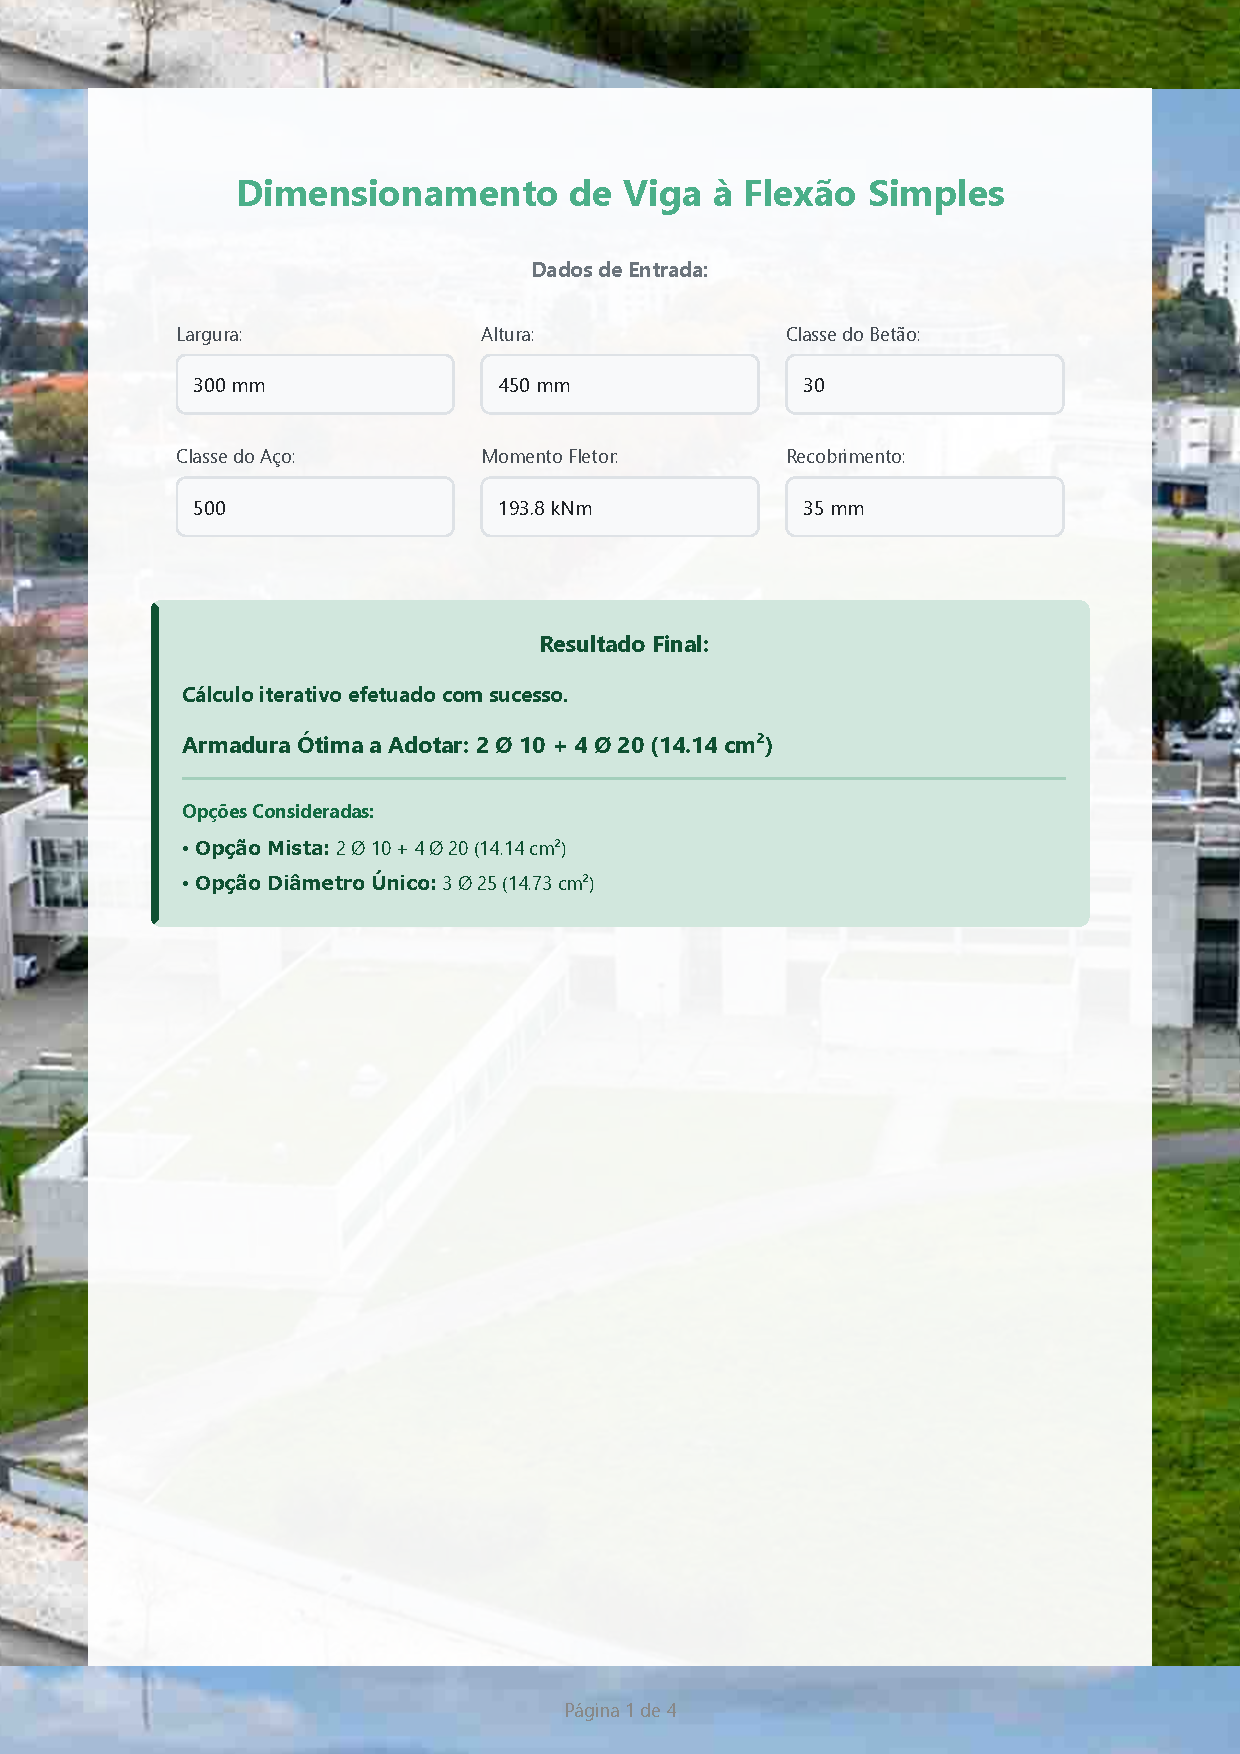
\includepdf[pages=-, pagecommand={}]{Anexos/Relatorio-de-Calculo-Estrutural-_-Viga.pdf}

% =========================================================
% APÊNDICE J
% =========================================================
\newpage
\addcontentsline{toc}{section}{APÊNDICE J - Resultado do dimensionamento do pilar}
\begin{center}
\section*{APÊNDICE J}
Resultado do dimensionamento do pilar
\end{center}

O documento seguinte apresenta o resultado do dimensionamento do pilar gerado pela aplicação para o caso de validação correspondente.

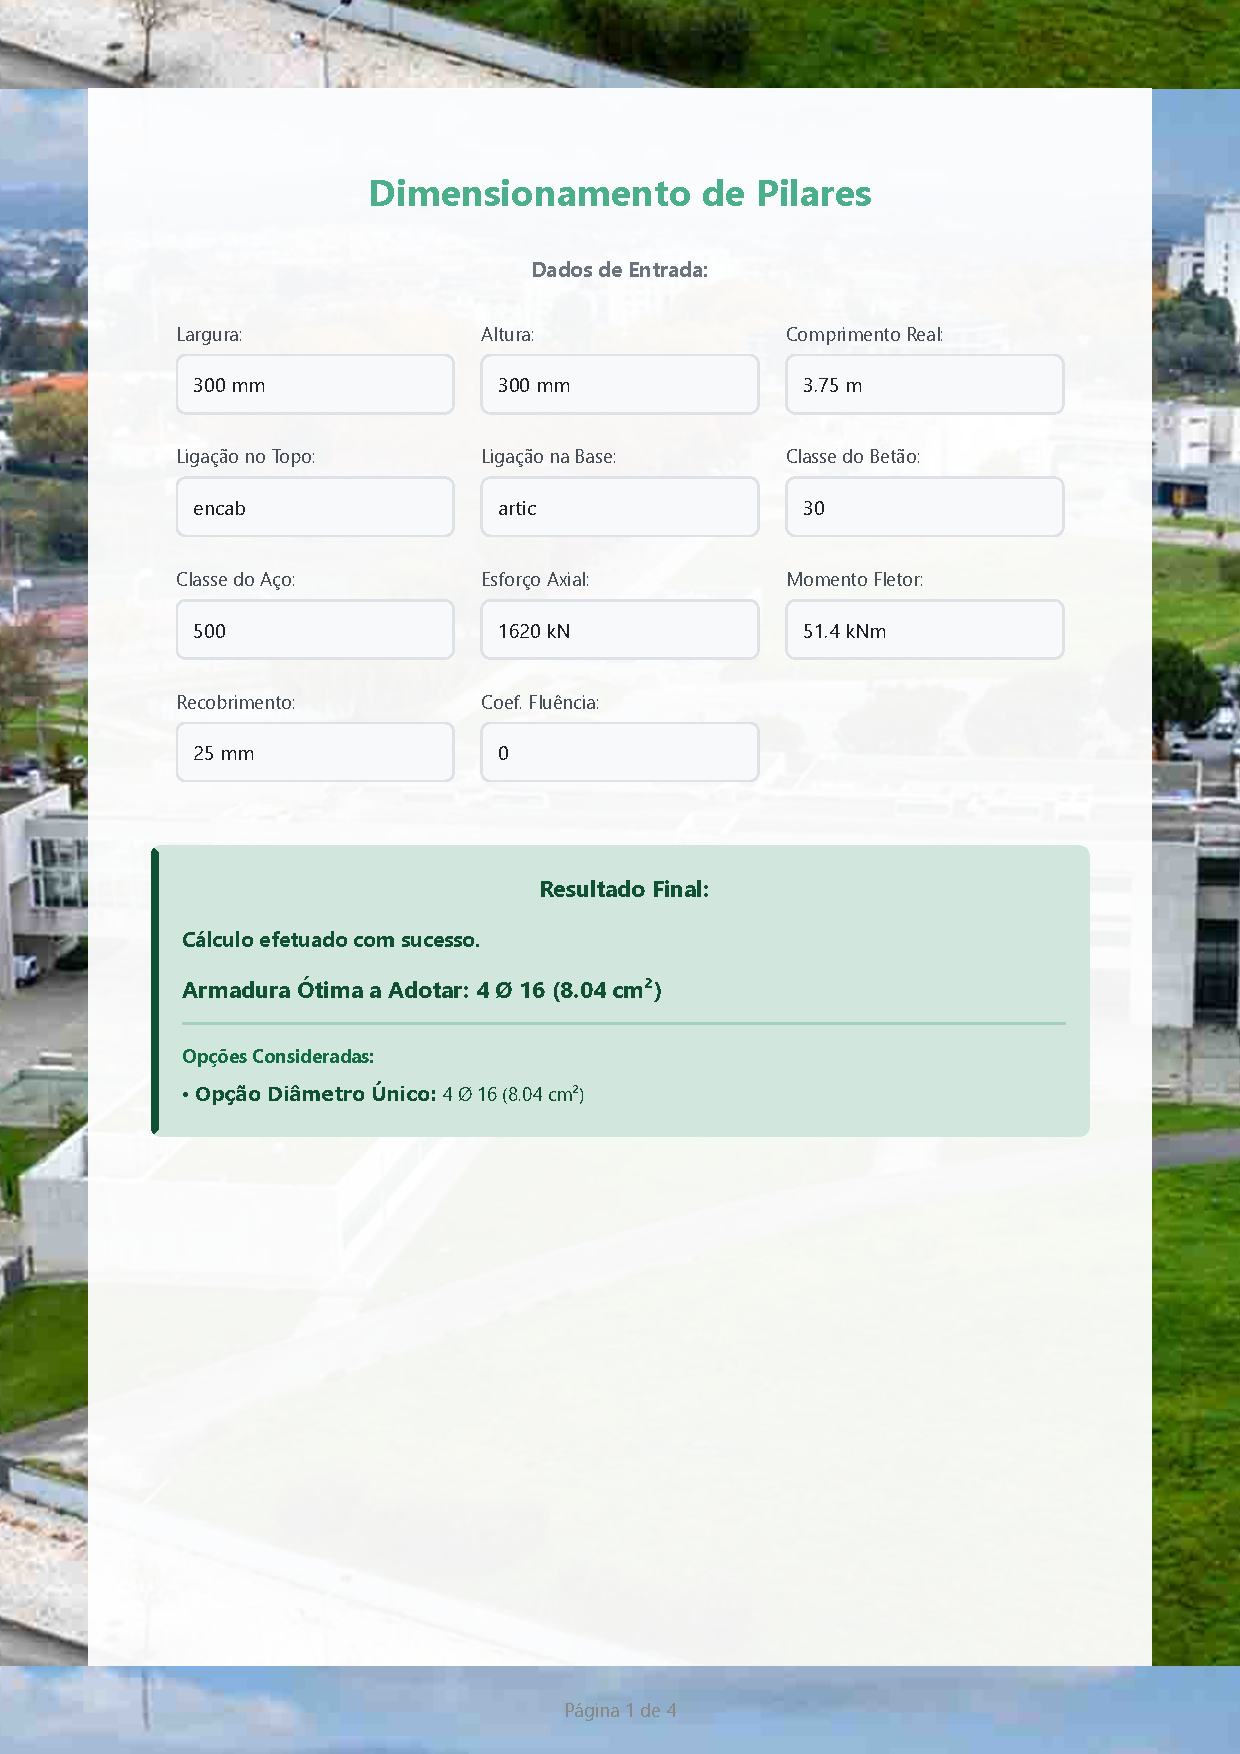
\includepdf[pages=-, pagecommand={}]{Anexos/Relatorio-de-Calculo-Estrutural-_-Pilar-2.pdf}

% =========================================================
% APÊNDICE K
% =========================================================
\newpage
\addcontentsline{toc}{section}{APÊNDICE K - Resultado do dimensionamento da sapata}
\begin{center}
\section*{APÊNDICE K}
Resultado do dimensionamento da sapata
\end{center}

O documento seguinte apresenta o resultado do dimensionamento da sapata gerado pela aplicação para o caso de validação correspondente.

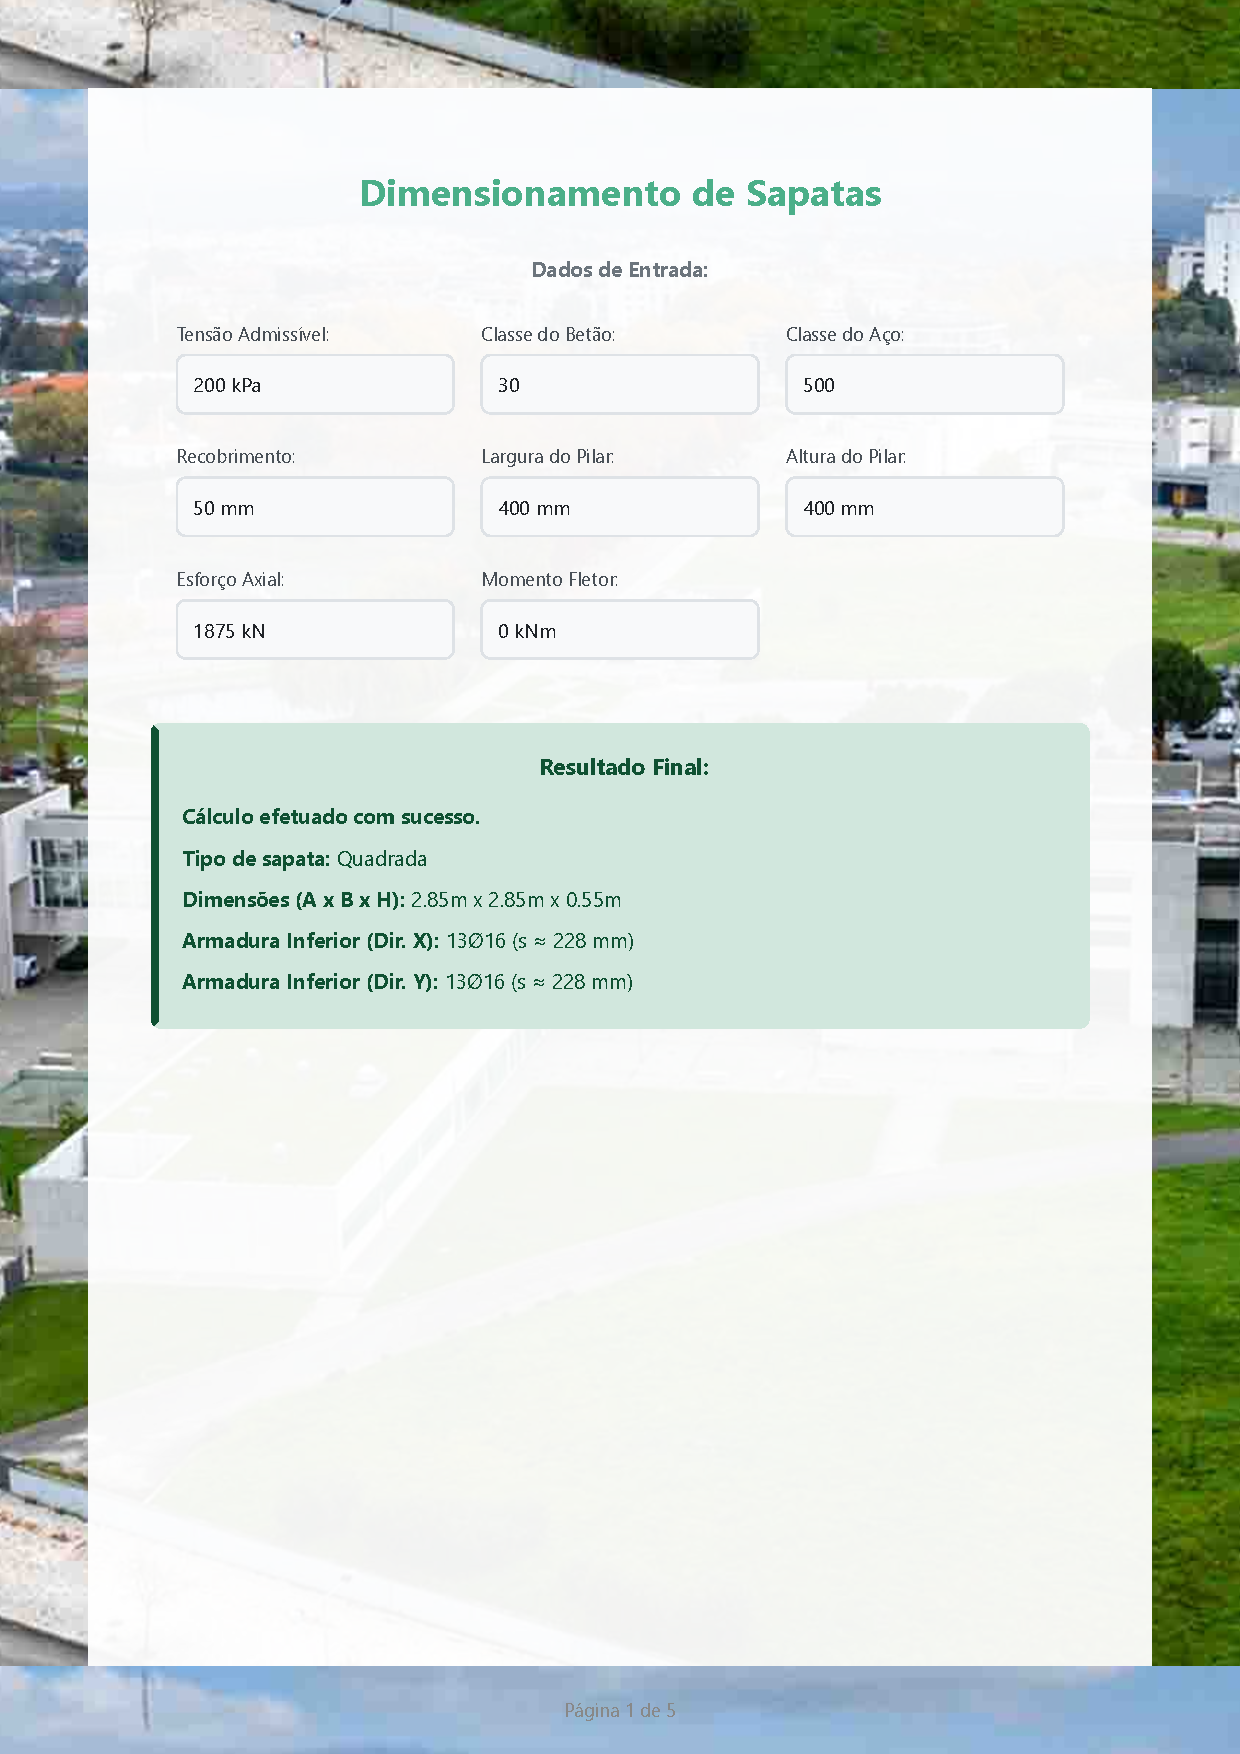
\includepdf[pages=-, pagecommand={}]{Anexos/Relatorio-de-Calculo-Estrutural-_-Sapata-3.pdf}